\let\negmedspace\undefined
\let\negthickspace\undefined
\documentclass[article]{IEEEtran}
\usepackage[a5paper, margin=10mm, onecolumn]{geometry}
\usepackage{tfrupee}

\setlength{\headheight}{1cm}
\setlength{\headsep}{0mm}

\usepackage{gvv-book}
\usepackage{gvv}
\usepackage{cite}
\usepackage{amsmath,amssymb,amsfonts,amsthm}
\usepackage{algorithmic}
\usepackage{graphicx}
\usepackage{textcomp}
\usepackage{xcolor}
\usepackage{txfonts}
\usepackage{listings}
\usepackage{enumitem}
\usepackage{mathtools}
\usepackage{gensymb}
\usepackage{comment}
\usepackage[breaklinks=true]{hyperref}
\usepackage{tkz-euclide} 
\usepackage{listings}                                       
\def\inputGnumericTable{}                                 
\usepackage[latin1]{inputenc}                                
\usepackage{color}                                            
\usepackage{array}                                            
\usepackage{longtable}                                       
\usepackage{calc}                                             
\usepackage{multirow}                                         
\usepackage{hhline}                                           
\usepackage{ifthen}                                           
\usepackage{lscape}

\renewcommand{\thefigure}{\theenumi}
\renewcommand{\thetable}{\theenumi}
\setlength{\intextsep}{10pt}

\numberwithin{figure}{enumi}
\renewcommand{\thetable}{\theenumi}
\begin{document}
\bibliographystyle{IEEEtran}
\title{NCERT-12.6.5.1.2}
\author{EE24BTECH11035 - KOTHAPALLI AKHIL}
{\let\newpage\relax\maketitle}
\noindent\textbf{Question: }  
Finding Minimum and Maximum Values of $y = 9x^2 + 12x + 2$.\\
\solution \\
\textbf{Theoretical Method:}\\
We aim to find the minimum and maximum values of the quadratic function $y = 9x^2 + 12x + 2$. First, we calculate the first derivative of $y$ with respect to $x$:

\begin{align}
\frac{dy}{dx} &= 18x + 12
\end{align}

Setting the derivative equal to zero, we find the critical points:

\begin{align}
18x + 12 &= 0 \\
x &= -\frac{2}{3}
\end{align}

To determine whether this critical point is a minimum or maximum, we compute the second derivative:

\begin{align}
\frac{d^2y}{dx^2} &= 18
\end{align}

Since $\frac{d^2y}{dx^2} > 0$, the function has a minimum at $x = -\frac{2}{3}$. Now, we calculate the corresponding $y$ value:

\begin{align}
y &= 9\left(-\frac{2}{3}\right)^2 + 12\left(-\frac{2}{3}\right) + 2 \\
&= 9 \times \frac{4}{9} - 8 + 2 \\
&= 4 - 8 + 2 \\
&= -2
\end{align}

Thus, the minimum value of $y$ is $-2$ at $x = -\frac{2}{3}$. Since the parabola opens upwards, it has no maximum value as $x \to \infty$.

\noindent\textbf{Computational Method:}\\
Find the Derivative,\\
The derivative of the function $f(x) = 9x^2 + 12x + 2$ is:
\begin{align}
f'(x) &= 18x + 12
\end{align}
The gradient descent update rule is:
\begin{align}
x_{n+1} &= x_n - \mu f'(x_n)
\end{align}
Substituting the derivative:
\begin{align}
x_{n+1} &= x_n - \mu (18x_n + 12)
\end{align}
Simplifying:
\begin{align}
x_{n+1} &= (1 - 18\mu)x_n - 12\mu
\end{align}
Express as a Difference Equation,\\
Rewrite the update rule as:
\begin{align}
x_{n+1} - (1 - 18\mu)x_n &= -12\mu
\end{align}
Taking the Z-transform of both sides:
\begin{align}
zX(z) - zx_0 &= (1 - 18\mu)X(z) - 12\mu \frac{z}{z-1}
\end{align}
Rearrange to solve for $X(z)$:
\begin{align}
(z - (1 - 18\mu))X(z) &= zx_0 - 12\mu \frac{z}{z-1}
\end{align}
\begin{align}
X(z) &= \frac{zx_0 - 12\mu \frac{z}{z-1}}{z - (1 - 18\mu)}
\end{align}
\begin{align}
X(z) = \frac{zx_0}{z - (1 - 18\mu)}-\frac{12\mu \frac{z}{z-1}}{z - (1 - 18\mu)}
\end{align}
The ROC determined for stability condition:
\begin{align}
    |1-18\mu|<1
\end{align}
\begin{align}
    -1<1-18\mu<1
\end{align}
\begin{align}
    0<18\mu<2 
\end{align}
\begin{align}
    0<\mu<\frac{1}{9}
\end{align}
If $\mu$ satisfies the above given condition then,
\begin{align}
    \lim_{n\rightarrow\infty}\norm{x_{n+1}-x_n}=0\\
    \implies \lim_{n\rightarrow\infty}\norm{\mu\brak{-12-18x_n}}=0\\
    \implies -12\mu-18\mu\lim_{x\rightarrow\infty}\norm{x_n}=0\\
    \implies \lim_{x\rightarrow\infty}\norm{x_n}=-\frac{2}{3}
\end{align}
Taking initial guess of $x=0$\\
step-size = 0.01\\
Tolerence = 1e-6\\
we get ,\\
$x=-0.6666$\\
\textbf{Using Quadratic programming :}\\
Find the point lying on the line $y = 1$, which is nearest to the origin.

We can formulate the problem as follows:
\begin{align}
    &\min_{\mathbf{x}} \|e_2^T \mathbf{x}\|^2 \\
    &\text{s.t.} \\
    &\mathbf{x}^T \mathbf{V} \mathbf{x} + 2 \mathbf{u}^T \mathbf{x} + f = 0
\end{align}

where
\begin{align}
    \mathbf{V} &= \begin{bmatrix} 4 & 0 \\
    0 & 0 \end{bmatrix}, \\
    \mathbf{u} &= \begin{bmatrix} -2 \\
    0 \end{bmatrix}, \\
    f &= 4.
\end{align}

In the current form, the constraint is non-convex since the constraint defines a set which is not convex. Points on the line joining any two points on the curve do not belong to the set. However, if we relax the constraint and make it:
\begin{align}
    \mathbf{x}^T \mathbf{V} \mathbf{x} + 2 \mathbf{u}^T \mathbf{x} \leq 0,
\end{align}

then the constraint becomes convex.

Using \texttt{cvxpy} to solve this convex optimization problem, we obtain the solution for the general quadratic programming formulation. \\
We rewrite the quadratic expression $9x^2 + 12x + 2$ as a standard quadratic programming problem. The objective function is given by:
\begin{align}
    &\min \ 9x^2 + 12x + 2,
\end{align}
subject to specific constraints derived from the problem context.

Using the methods described above and implementing them in \texttt{cvxpy}, the optimization problem can be solved efficiently.
\begin{figure}[h!]
	\centering
	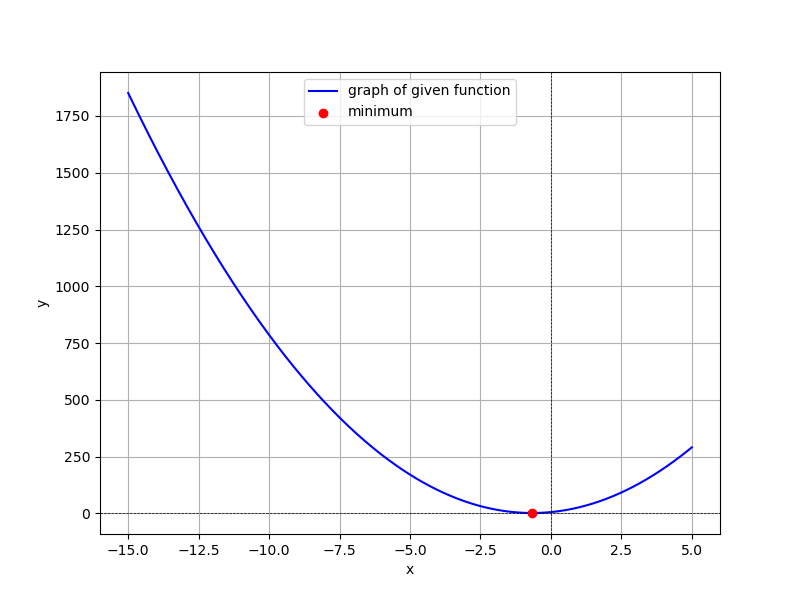
\includegraphics[width=\columnwidth]{figures/Figure_1.png}
	\caption{Graph of given quadratic function}
	\label{stemplot}
\end{figure}
\end{document}

